This chapter covers the training and evaluation of the HighRes-net super-resolution network trained with different datasets.
Various training possibilities are explored in regard to the network generalization problem.
The end of the chapter presents and discusses the summarized results.

\section{Training HighRes-net}
As stated in the experiment layout, the final step consists in training HighRes-net super-resolution model with different data.
One final step before conducting the training is to examine visually the results of augmentation on a Sentinel-2 image.
These are presented for the all the augmentation network architectures in Figures \ref{fig:export-example} and \ref{fig:export-example-zoomed}.
\begin{figure}
    \begin{subfigure}[t]{0.3\textwidth}
        \centering
        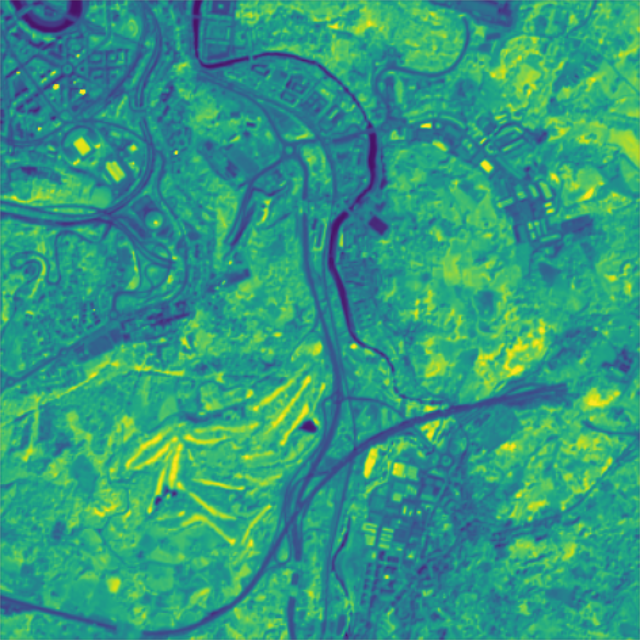
\includegraphics[width=\textwidth]{sentinel_export_hr}
        \caption{High-resolution}
    \end{subfigure}
    \hfill
    \begin{subfigure}[t]{0.3\textwidth}
        \centering
        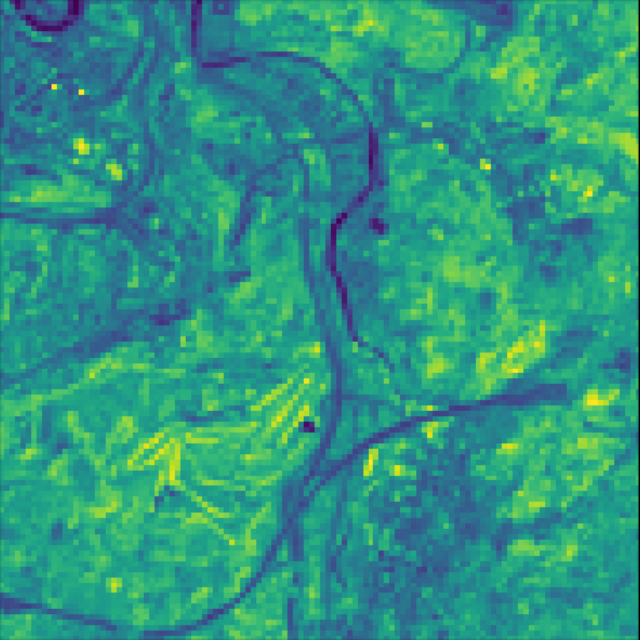
\includegraphics[width=\textwidth]{sentinel_export_bicubic}
        \caption{Low-resolution image created from the high-resolution one with bicubic interpolation}
    \end{subfigure}
    \hfill
    \begin{subfigure}[t]{0.3\textwidth}
        \centering
        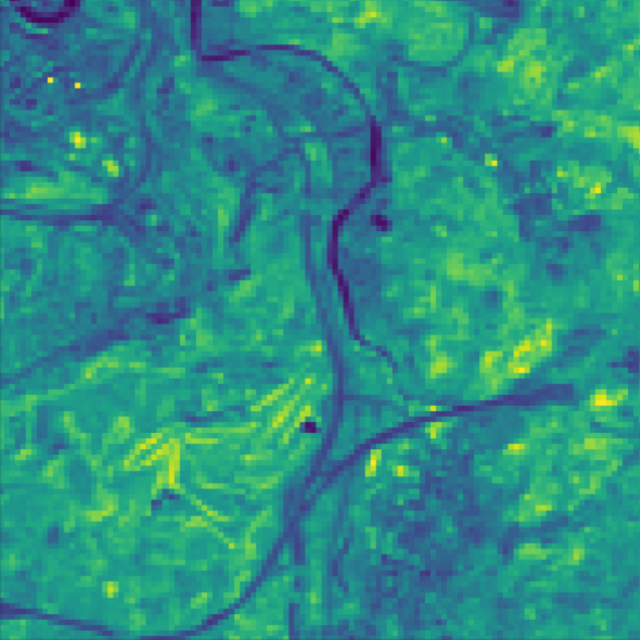
\includegraphics[width=\textwidth]{sentinel_export_simple_conv}
        \caption{Low-resolution image created from the high-resolution one by the simple convolutional network}
    \end{subfigure}
    \hfill
    \medskip
    \centering
    \hfill
    \begin{subfigure}[t]{0.3\textwidth}
        \centering
        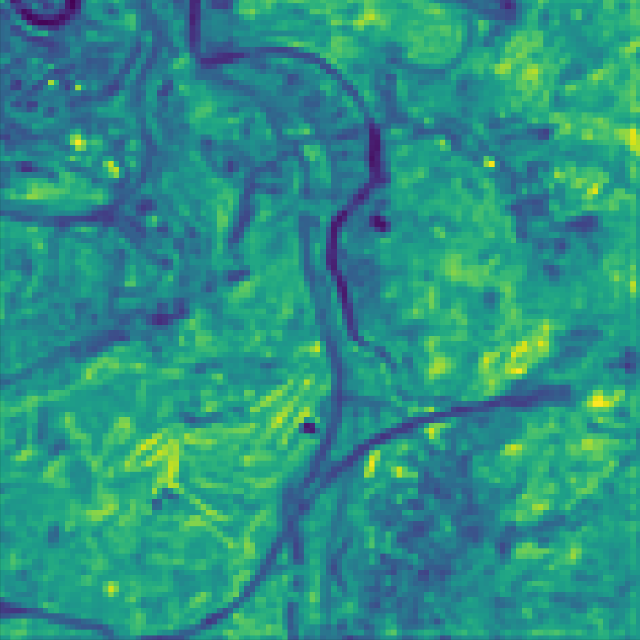
\includegraphics[width=\textwidth]{sentinel_export_autoencoder}
        \caption{Low-resolution image created from the high-resolution one by the encoder-decoder network}
    \end{subfigure}
    \quad
    \begin{subfigure}[t]{0.3\textwidth}
        \centering
        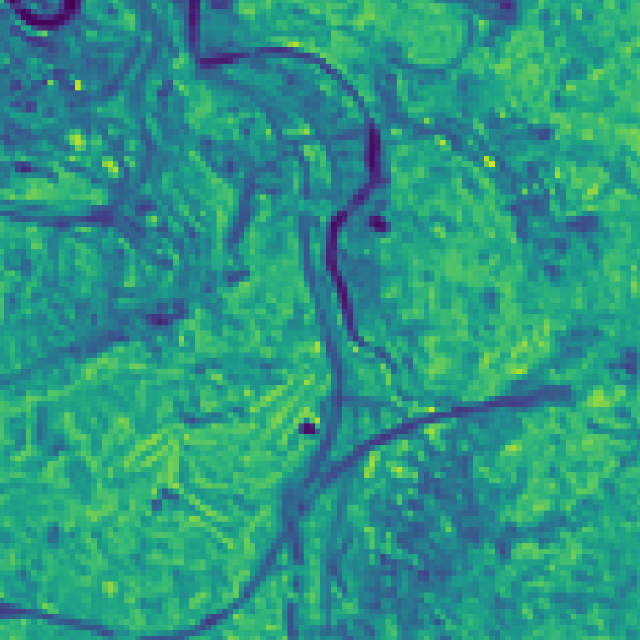
\includegraphics[width=\textwidth]{sentinel_export_gan}
        \caption{Low-resolution image created from the high-resolution one by the \gls{gan} network}
    \end{subfigure}
    \hfill
    \caption{Example of Sentinel-2 training dataset images created in different ways}
    \label{fig:export-example}
\end{figure}
\begin{figure}
        \begin{subfigure}[t]{0.3\textwidth}
        \centering
        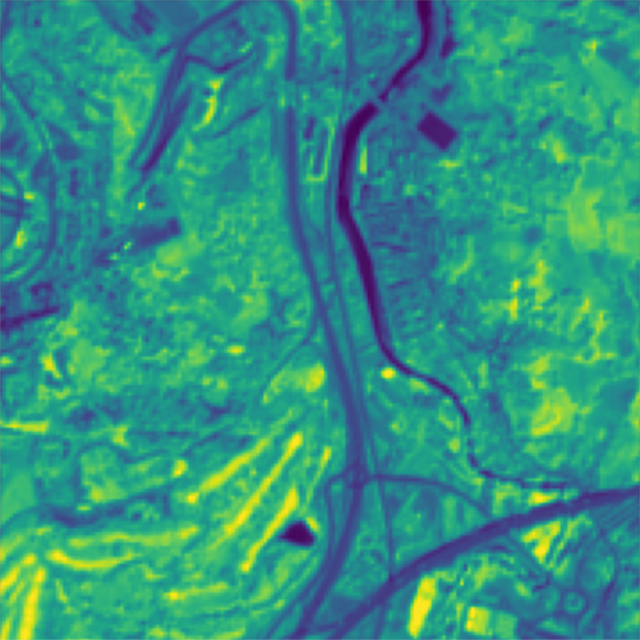
\includegraphics[width=\textwidth]{sentinel_export_zoomed_hr}
        \caption{High-resolution}
    \end{subfigure}
    \hfill
    \begin{subfigure}[t]{0.3\textwidth}
        \centering
        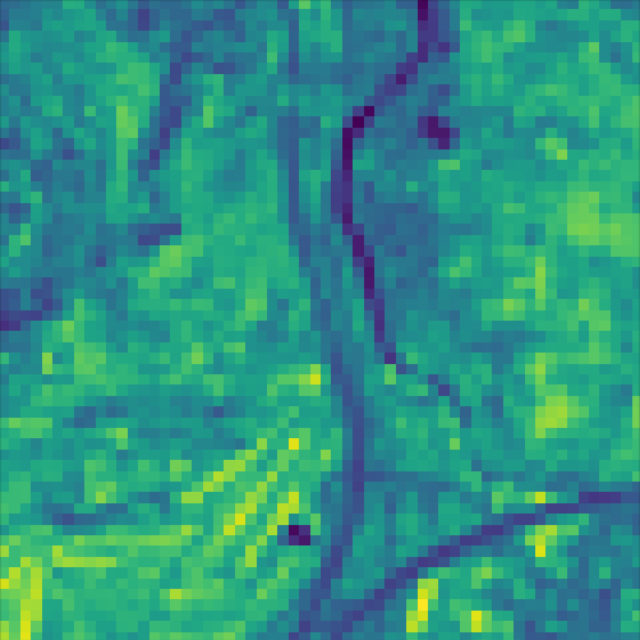
\includegraphics[width=\textwidth]{sentinel_export_zoomed_bicubic}
        \caption{Low-resolution image created from the high-resolution one with bicubic interpolation}
    \end{subfigure}
    \hfill
    \begin{subfigure}[t]{0.3\textwidth}
        \centering
        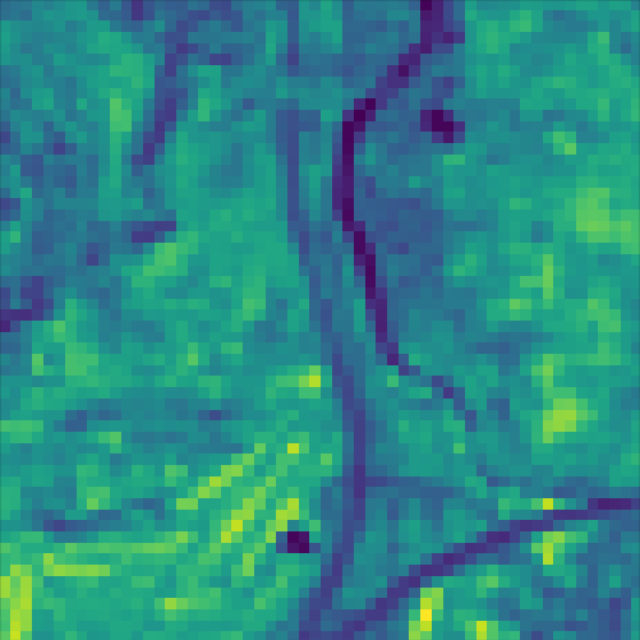
\includegraphics[width=\textwidth]{sentinel_export_zoomed_simple_conv}
        \caption{Low-resolution image created from the high-resolution one by the simple convolutional network}
    \end{subfigure}
    \hfill
    \medskip
    \centering
    \hfill
    \begin{subfigure}[t]{0.3\textwidth}
        \centering
        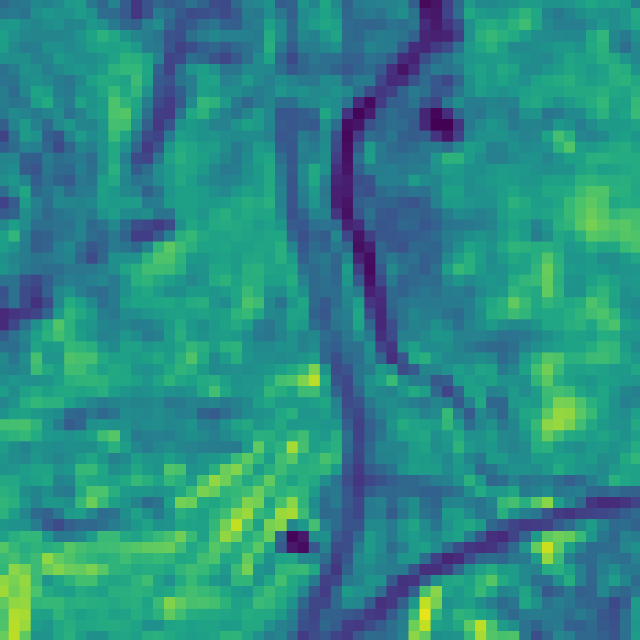
\includegraphics[width=\textwidth]{sentinel_export_zoomed_autoencoder}
        \caption{Low-resolution image created from the high-resolution one by the encoder-decoder network}
    \end{subfigure}
    \quad
    \begin{subfigure}[t]{0.3\textwidth}
        \centering
        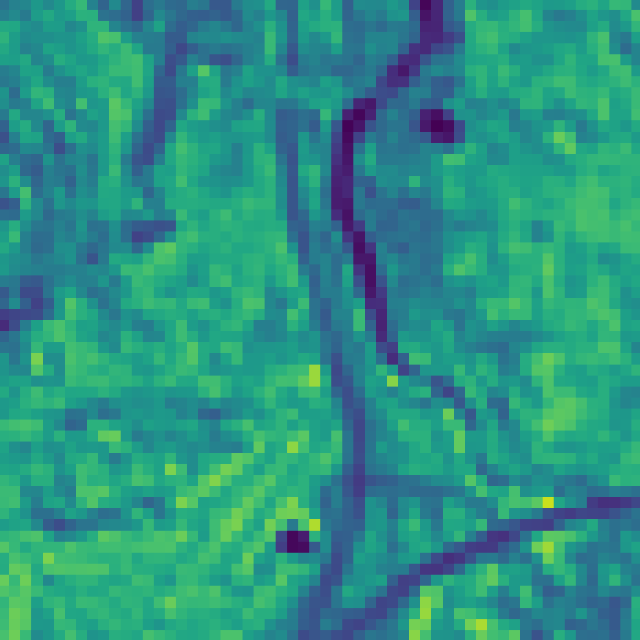
\includegraphics[width=\textwidth]{sentinel_export_zoomed_gan}
        \caption{Low-resolution image created from the high-resolution one by the \gls{gan} network}
    \end{subfigure}
    \hfill
    \caption{Zoomed examples of Sentinel-2 training dataset images created in different ways}
    \label{fig:export-example-zoomed}
\end{figure}

It should be kept in mind, that the training dataset created by resizing with bicubic interpolation was subject to additional transformations of contrast, noise, and blur as stated in Chapter \ref{ch:scope}.

As planned, the super-resolution is to be trained with multi-image data in a single-band (band eight) mode.
Training is configured in such a way that only weights for the best validation score are saved.
However, automatic stopping is not enabled.
For this reason, fitting was interrupted manually around epoch 100 when all training curves plateaued.
The training history has been plotted to visualize the fitting progress.
Figure \ref{fig:highres-net-training-loss} shows the loss history for all discussed HighRes-net trainings, Figure \ref{fig:highres-net-training-validation} presents the validation loss improvement.
Section \ref{sec:cross-type} discusses some parts of these figures in a more detailed way. 

\subsection{Stop condition based on cross-data-type validation}
\label{sec:cross-type}
Having multiple datasets generated in different ways enables an alternative way of validating the super-resolution training process.
Instead of taking a subpart of the training set as validation data, one may use images generated in a different way.
Such a technique may help to investigate the generalization capabilities of the super-resolution network.
This kind of validation is available thanks to the multiplicity of the generated datasets and is unique to this work.
The dataset created using the simple convolutional network and resizing algorithm were used for the cros-type-validation.
In this scheme the training and validation sets are created in different ways which enables broader look on evaluation during training.
It should be noticed, that the validation subsets were taken from the training datasets and not the evaluation test sets to prevent data leaks.
In Figures \ref{fig:highres-net-training-loss} and \ref{fig:highres-net-training-validation}, in the case of the cross-data-type validation scheme, the letter \textit{t} denotes the training dataset and the letter \textit{v} denotes the validation dataset.
When using the cross-data-type evaluation the validation loss stops to decrease significantly earlier, as seen in Figure \ref{fig:highres-net-training-validation}.
A small raise in validation loss is visible for over ten epochs before the training was stopped.
In this case, the best weights were saved nearly three times earlier than during the non-cross-type-validated training. 
This may indicate that the vast part of the fitting process does not contribute to the overall generalization capability of the super-resolution network.
The cross-validated training is stopped earlier; since only weights for the epoch with the best validation score are saved, it is pointless to run longer fittings.
\begin{figure}
    \centering
    \begin{tikzpicture}
			\begin{axis}[width=\linewidth, height=12cm, xmin=-9.9, xmax=110, legend cell align={left}, ymode=log, grid=major, grid style={dashed}, xlabel=Epoch, ylabel=Loss]
			\addlegendentry{Bicubic}
			\addplot+[mark=none] table [x=step, y=value, col sep=comma] {data/highresnet_s2ab_ab5_bb8_20210608-114450-training_loss.csv};
			\addlegendentry{Simple convolutional}
						\addplot+[mark=none] table [x=step, y=value, col sep=comma] {data/highresnet_s2_degraded_simple_conv-dvc-21-07-04_044726_e34_bb8_20210706-183639-training_loss.csv};
			\addlegendentry{Encoder-decoder}
						\addplot+[mark=none] table [x=step, y=value, col sep=comma] {data/highresnet_s2_degraded_autoencoder-dvc-21-07-04-052647_e23_bb8_20210707-100146-training_loss.csv};
			\addlegendentry{\gls{gan}}
						\addplot+[mark=none] table [x=step, y=value, col sep=comma] {data/highresnet_s2_degraded-gan-dvc-21-07-04-055506_e94_bb8_20210707-152641-training_loss.csv};
			\addlegendentry{t: Bicubic, v: Simple convolutional}
						\addplot+[mark=none, color=green] table [x=step, y=value, col sep=comma] {data/highresnet_s2ab_ab5_bb8_20210726-160215-training_loss.csv};

			\end{axis}		\end{tikzpicture}
    \caption{HighRes-net training loss history with training sets created in different ways}
    \label{fig:highres-net-training-loss}
\end{figure}
\begin{figure}
    \centering
    \begin{tikzpicture}
			\begin{axis}[width=\linewidth, height=12cm, xmin=-9.9, xmax=110, legend cell align={left}, grid=major, grid style={dashed}, xlabel=Epoch, ylabel=Loss]
			\addlegendentry{Bicubic}
			\addplot+[mark=none] table [x=step, y=value, col sep=comma] {data/highresnet_s2ab_ab5_bb8_20210608-114450-validation_loss.csv};
			\addlegendentry{Simple convolutional}
						\addplot+[mark=none] table [x=step, y=value, col sep=comma] {data/highresnet_s2_degraded_simple_conv-dvc-21-07-04_044726_e34_bb8_20210706-183639-validation_loss.csv};
			\addlegendentry{Encoder-decoder}
						\addplot+[mark=none] table [x=step, y=value, col sep=comma] {data/highresnet_s2_degraded_autoencoder-dvc-21-07-04-052647_e23_bb8_20210707-100146-validation_loss.csv};
			\addlegendentry{\gls{gan}}
						\addplot+[mark=none] table [x=step, y=value, col sep=comma] {data/highresnet_s2_degraded-gan-dvc-21-07-04-055506_e94_bb8_20210707-152641-validation_loss.csv};
			\addlegendentry{t: Bicubic, v: Simple convolutional}
						\addplot+[mark=none, color=green] table [x=step, y=value, col sep=comma] {data/highresnet_s2ab_ab5_bb8_20210726-160215-validation_loss.csv};

			\end{axis}		\end{tikzpicture}
    \caption{HighRes-net validation loss history with training sets created in different ways}
    \label{fig:highres-net-training-validation}
\end{figure}

\section{Evaluation and results}
According to the experiment layout, the trained super-resolution models are to be evaluated on a variety of test datasets to examine generalization capabilities and robustness.
As stated before, the evaluation datasets include:
\begin{itemize}
	\item Test subsets from all augmented Sentinel-2 datasets that can be used for calculating numerical metrics.
	\item Real-life Sentinel-2 images that were not used in the training process and do not include high and low-resolution pairs, so only visual examination can be performed. These are original images that were not downsampled. This means that they have different resolution and \gls{gsd} than the low-resolution images in the artificial datasets used for training the super-resolution networks. 
	\item Proba-V original real-life test dataset that can be used for calculating numerical metrics.
\end{itemize}
It should be noticed, that the latter two test sets differ in the \gls{gsd} parameter from the synthetic low-resolution images in the Sentinel-2 training datasets.
This data is still valid for evaluation and investigation because it is desirable that super-resolution and machine learning algorithms in general work on objects of any scale and size.
Limiting the tests to a single \gls{gsd} would draw an incomplete picture of the results.
The results of the evaluation are presented in Table \ref{tab:super-res-results}, where rows designate test datasets and columns indicate models trained on data created in different ways.
For the cross-validation training scenarios, letters \textit{t} and \textit{v} indicate the training and validation datasets respectively.
The cPSNR score was used as the super-resolution evaluation metric.

The best results are observed along the diagonal of the table, which means that the super-resolution model works best on test data created in the same way as training data for a given model.
A visual demonstration of such an evaluation can be seen in Figure \ref{fig:highresnet-test-visual}.
In this case, HighRes-net was trained on the dataset created by the simple convolutional network and evaluated on the test subpart of the same dataset.
An example of image upscaling with bicubic interpolation was included in the figure as a reference point.
The best results along the diagonal are expected and indicate that no gross mistakes were made in the course of the work.
Each network works best on the data created in the same way as its training set.
The super-resolution network trained using data generated by the simple convolutional network recreates the original high-resolution images best (with cPSNR of 36.15).
\begin{figure}
    \centering
    \begin{subfigure}[t]{0.45\textwidth}
        \centering
        
\includegraphics[width=\textwidth]{highresnet_test_lr}
        \caption{One of nine low-resolution images}
    \end{subfigure}
    \hfill
    \begin{subfigure}[t]{0.45\textwidth}
        \centering
        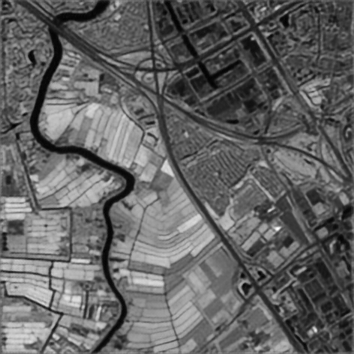
\includegraphics[width=\textwidth]{highresnet_test_sr}
        \caption{Super-resolution reconstruction of the scene}
    \end{subfigure}
    \begin{subfigure}[t]{0.45\textwidth}
        \centering
        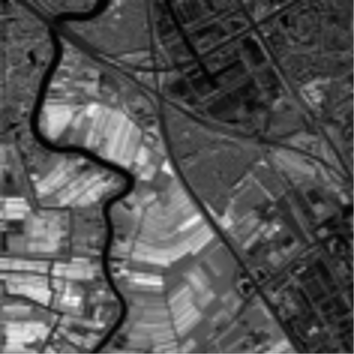
\includegraphics[width=\textwidth]{highresnet_test_bicubic}
        \caption{Upscaling to high-resolution with bicubic interpolation}
    \end{subfigure}
    \hfill
    \begin{subfigure}[t]{0.45\textwidth}
        \centering
        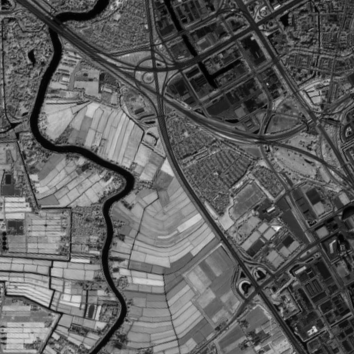
\includegraphics[width=\textwidth]{highresnet_test_hr}
        \caption{Real-life high-resolution picture of the scene}
    \end{subfigure}
    \caption{A visual example of evaluation of an augmented dataset; both the training and test datasets were generated using the simple convolutional network}
    \label{fig:highresnet-test-visual}
\end{figure}
\begin{table}
\caption{Evaluation of super-resolution training on different test sets (cPSNR metric, the larger, the better)}
\label{tab:super-res-results}
\begin{adjustbox}{center}
\small
\begin{tabular}{@{}llccccc@{}}
\toprule
\multicolumn{2}{c}{\multirow{2}{*}{}} & \multicolumn{5}{c}{\textbf{Training data}}                                             \\ \cmidrule{3-7} 
\multicolumn{2}{c}{} &
  Bicubic &
  Simple conv &
  Encoder-decoder &
  \gls{gan} &
  \begin{tabular}[c]{@{}c@{}}t: Bicubic\\ v: Simple conv\end{tabular} \\ \midrule
\multirow{5}{*}{\rotatebox[origin=c]{90}{\textbf{Test data}}} &
  Bicubic &
  \textbf{35.78} &
  28.96 &
  24.55 &
  25.80 &
  35.26 \\
           & Simple conv          & 33.69 & \textbf{36.15} & 27.16          & 29.83          & 33.67          \\
           & Encoder-decoder               & 31.72 & 31.78          & \textbf{34.43} & 30.22          & 31.76          \\
           & \gls{gan}                     & 28.63 & 28.63          & 27.27          & \textbf{35.72} & 30.28          \\
           & Proba-V                       & 43.36 & 42.02          & 40.43          & 40.91          & \textbf{43.51} \\ \bottomrule
\end{tabular}
\end{adjustbox}
\end{table}

As stated in Chapter \ref{ch:scope}, an additional set of original real-life Sentinel-2 images is available.
This set includes single-resolution images with different \gls{gsd} than the synthetic training datasets.
Since this set does not feature high and low-resolution image pairs, it can be used only for visual examination.
Samples for such visual evaluation are shown in Figure \ref{fig:sentinel-real-artifacts}.
Some mosaic or checkerboard-like artifacts can be observed in the super-resolved images.
As seen in the samples, some form of artifacts occurred for all the networks on real-life Sentinel-2 data (with higher \gls{gsd} than the training low-resolution images).
\begin{figure}
    \centering
    \begin{subfigure}[t]{0.32\textwidth}
        \centering
        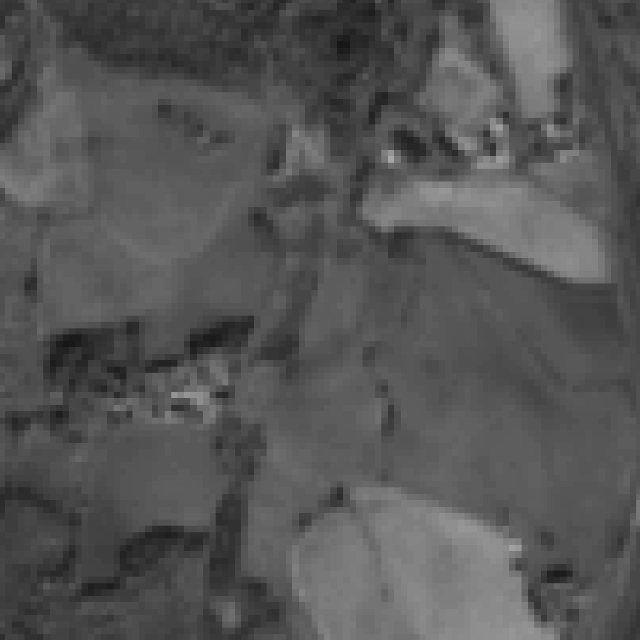
\includegraphics[width=\textwidth]{sentinel_real_lr}
        \caption{One of the low-resolution images of the test scene}
    \end{subfigure}
    \hfill
    \begin{subfigure}[t]{0.32\textwidth}
        \centering
        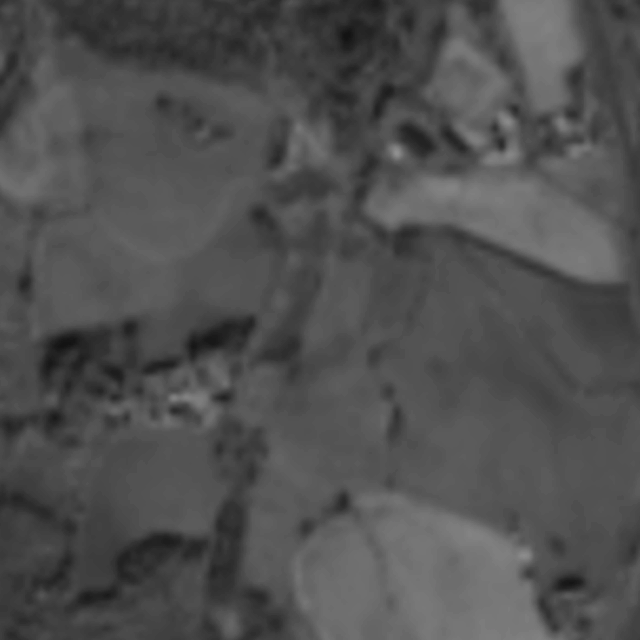
\includegraphics[width=\textwidth]{sentinel_real_upscale_bicubic} 
        \caption{Upscaling to high-resolution with bicubic interpolation}
    \end{subfigure}
    \hfill
    \begin{subfigure}[t]{0.32\textwidth}
        \centering
        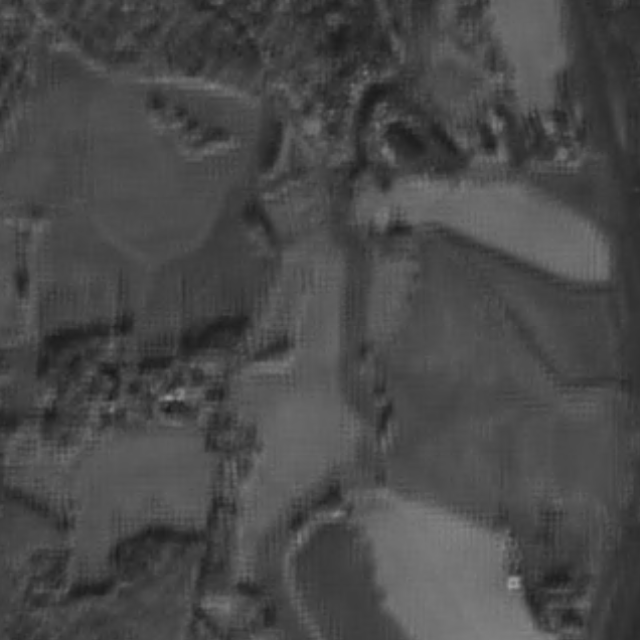
\includegraphics[width=\textwidth]{setinel_real_sr_bicubic}
        \caption{HigRes-net trained on data created with bicubic interpolation}
    \end{subfigure}
    \hfill
    \smallskip
    \centering
    \hfill
    \begin{subfigure}[t]{0.32\textwidth}
        \centering
        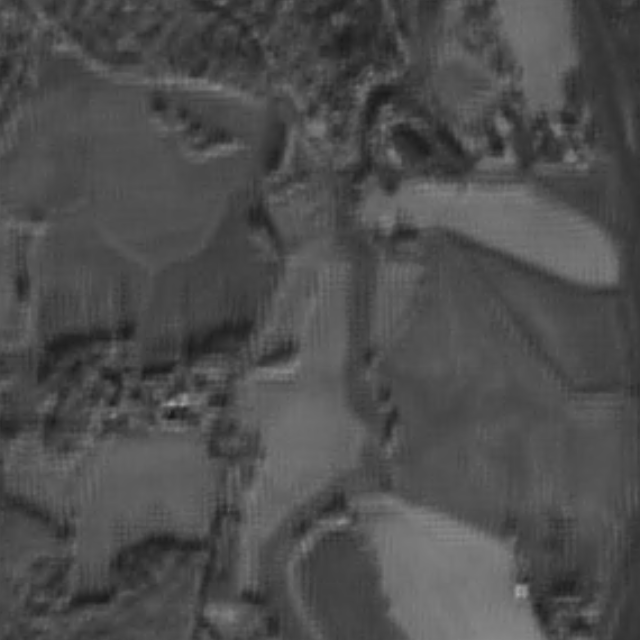
\includegraphics[width=\textwidth]{sentinel_real_sr_simple_tbic_vsimple}
        \caption{HigRes-net trained on data created with bicubic interpolation; training done with cross-data-type validation}
    \end{subfigure}
    \hfill
    \begin{subfigure}[t]{0.32\textwidth}
        \centering
         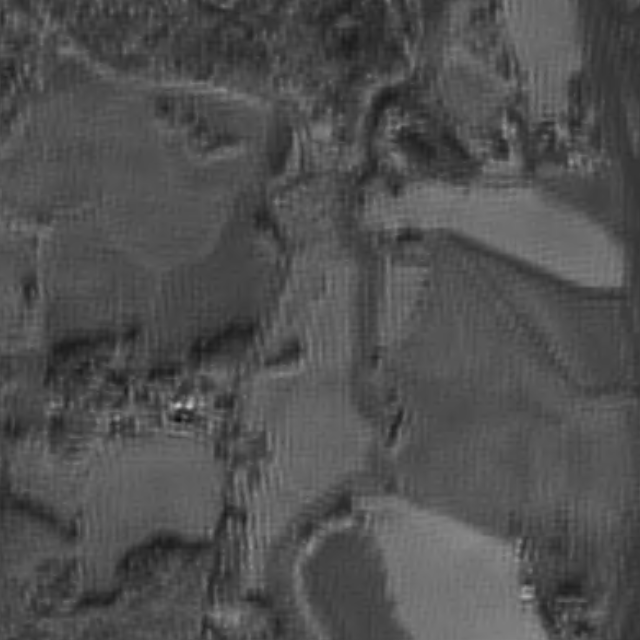
\includegraphics[width=\textwidth]{sentinel_real_sr_simple_conv}
        \caption{HigRes-net trained on data created by the simple conv network}
    \end{subfigure}
    \hfill
    \begin{subfigure}[t]{0.32\textwidth}
        \centering
        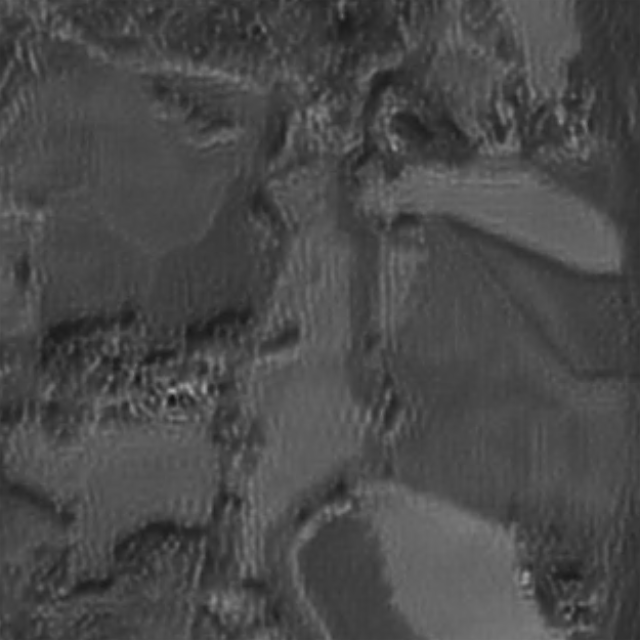
\includegraphics[width=\textwidth]{sentinel_real_sr_autoencoder}
        \caption{HigRes-net trained on data created by the encoder-decoder network}
    \end{subfigure}
    \hfill
    \smallskip
    \centering
    \hfill
    \begin{subfigure}[t]{0.32\textwidth}
        \centering
        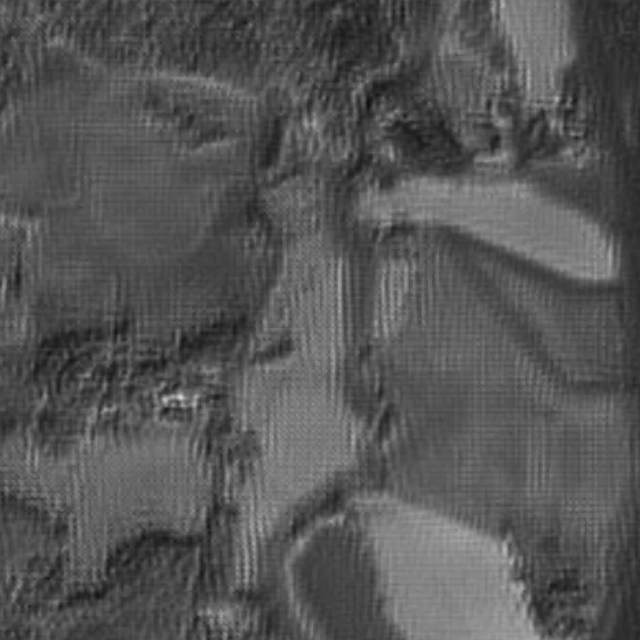
\includegraphics[width=\textwidth]{sentinel_real_sr_simple_gan}
        \caption{HigRes-net trained on data created by the \gls{gan} network}
    \end{subfigure}
    \hfill
    \captionsetup{justification=justified}
    \caption{A visual evaluation of super-resolution results on real-life Sentinel-2 test data. Images are super-resolved by HighRes-net trained on datasets created in different ways. One of the original low-resolution images and a high-resolution one created by upscaling with bicubic interpolation are added for reference.}
    \label{fig:sentinel-real-artifacts}
\end{figure}

The results in Table \ref{tab:super-res-results} and Figure \ref{fig:sentinel-real-artifacts} can be summarized in the following statements:
\begin{itemize}
	\item Data created with augmentation techniques, both traditional and deep learning-based is suitable for training super-resolution networks.
	\item The different deep learning architectures give fairly similar results, although the simplest one works best (achieves best results for the real-life Proba-V test subset).
	\item At the moment, the bicubic interpolation gives slightly better results for the real-life Proba-V test subset. Possible reasons for that and suggestions of improvement are included in the summary.
	\item The cross-data-type-validation proves that all trainings are prone to overfitting to the data generation techniques. Early stopping based on different datasets can lead to this conclusion. Using cross-data-type-validation resulted in a network that was trained for fewer epochs, yet performed slightly better on the real-life Proba-V test subset.
	\item The generalization capabilities of the networks trained on synthetic data pose a problem. Artifacts on real data can be observed.
\end{itemize}